% A partir da raiz do projeto: latexmk -pdf relatorio.tex
\PassOptionsToPackage{hypertexnames=false}{hyperref}
\documentclass[12pt,a4paper,oneside,openany,brazil,chapter=TITLE,section=TITLE]{abntex2}

\usepackage[T1]{fontenc}
\usepackage[utf8]{inputenc}
\usepackage{mathptmx}
\usepackage{indentfirst}
\usepackage{float}
\usepackage{microtype}
\usepackage{tikz}
\usetikzlibrary{arrows.meta}
\usepackage[alf,abnt-emphasize=bf,
  abnt-full-initials=yes,abnt-url-package=url]{abntex2cite}
\newcommand{\urlBibliografia}[1]{\href{#1}{#1}}
\AddToHook{cmd/thebibliography/after}{\let\url\urlBibliografia}

\setheadfoot{2cm}{1cm}
\setlength{\headsep}{1cm}
\checkandfixthelayout
\setlength{\parindent}{1.5cm}
\setlength{\parskip}{0pt}
\renewcommand{\ABNTEXchapterfont}{\bfseries}
\renewcommand{\ABNTEXchapterfontsize}{\normalsize}
\renewcommand{\ABNTEXsectionfont}{\normalfont}
\renewcommand{\ABNTEXsectionfontsize}{\normalsize}
\setlength{\afterchapskip}{1.5em}
\setlength{\aftersecskip}{0.9em}
\captionnamefont{\footnotesize}
\captiontitlefont{\footnotesize}
\makepagestyle{relatorio}
\makeoddhead{relatorio}{}{}{\footnotesize\thepage}

\titulo{Assinatura Digital e Execução Segura de Código}
\autor{Geovane Martins Schmitz\texorpdfstring{\\}{, }
  Otávio Augusto de Santana Jatobá\texorpdfstring{\\}{, }
  Vinicius Becker de Souza}
\local{Florianópolis}
\data{2026}
\hypersetup{hidelinks,pdftitle={\imprimirtitulo},pdfauthor={\imprimirautor}}

\begin{document}
\citeoption{autor-data}
\renewcommand{\bibname}{Referências Bibliográficas}
\pretextual
\begin{capa}
  \begin{center}
    UNIVERSIDADE FEDERAL DE SANTA CATARINA\par
    CENTRO TECNOLÓGICO\par
    DEPARTAMENTO DE INFORMÁTICA E ESTATÍSTICA\par
    CIÊNCIA DA COMPUTAÇÃO\par
    \vspace*{4cm}
    \imprimirautor\par
    \vspace*{5cm}
    \textbf{\imprimirtitulo}\par
    \vfill
    \imprimirlocal\par
    \imprimirdata\par
    \vspace*{1cm}
  \end{center}
\end{capa}
\setcounter{page}{1}
\textual
\pagestyle{relatorio}

\chapter{Introdução}

Como decidir se um kernel pode executar quando alguém pode alterar os arquivos
de inicialização? Essa decisão antecede as proteções do sistema operacional.
Escolhemos o Secure Boot para observar cada verificação de assinatura no
simulador e o momento em que o firmware autoriza a execução do Linux na VM.

\section{Funções de hash criptográfico}

Uma função de hash criptográfico transforma uma entrada de tamanho variável em um
resumo de tamanho fixo. Entre seus requisitos de segurança estão a resistência à
pré-imagem, à segunda pré-imagem e a colisões, tornando computacionalmente inviável
recuperar uma entrada a partir de seu resumo ou encontrar entradas distintas com o
mesmo resultado~\cite{stallings,stinson}. Este projeto utiliza a
função SHA-256.

\section{Assinaturas digitais}

As assinaturas digitais permitem verificar a integridade de uma mensagem e
associá-la ao detentor de uma chave privada. Na assinatura de código, o
signatário utiliza a chave privada e o resumo criptográfico do conteúdo.
O verificador utiliza a chave pública correspondente~\cite{stallings}.

\begin{figure}[H]
  \centering
  \caption{Criação de uma assinatura digital}
  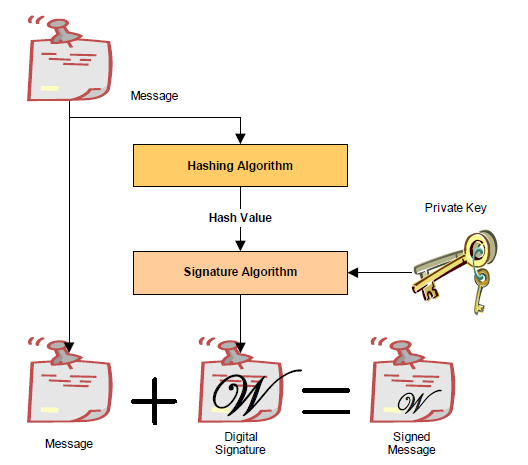
\includegraphics[width=0.38\linewidth]{figuras/assinatura-digital.png}
  \fonte{\citeonline{uefi}, \href{https://uefi.org/specs/UEFI/2.11/32_Secure_Boot_and_Driver_Signing.html\#creating-a-digital-signature}{\textit{Creating a Digital Signature}}.}
\end{figure}

\section{Raiz de confiança (Root of Trust)}

A raiz de confiança é o conjunto mínimo de componentes e informações cuja
confiabilidade constitui o ponto de partida da inicialização segura. Ela fornece
o código inicial de verificação e as referências criptográficas necessárias para
autenticar os componentes seguintes~\cite{zimmer}. Em uma implementação real de
Secure Boot, essa base pode incluir código protegido em hardware, como uma
memória de somente leitura~\cite{nist}.

\chapter{Assinatura Digital de Código}

\section{Processo de assinatura de executáveis}

Na VM, a assinatura integra o executável EFI que o firmware carrega~\cite{uefi}.
No simulador, o signatário assina um manifesto com RSA-PSS. O esquema incorpora
um valor aleatório (\textit{salt}), de modo que duas assinaturas válidas do
mesmo manifesto podem diferir~\cite{rfc8017}.

\section{Processo de verificação de assinaturas}

No simulador, o manifesto do kernel registra o SHA-256 esperado para esse
arquivo. Primeiro, o verificador usa a chave pública autorizada para conferir
a assinatura do manifesto. Em seguida, calcula o SHA-256 dos bytes do kernel
recebido e compara o resultado com o valor registrado. Se os dois resumos
coincidem, o verificador aceita o kernel descrito no manifesto autenticado.

Na VM, o firmware verifica a assinatura da imagem EFI e consulta suas bases de
confiança para decidir se pode executar a imagem~\cite{uefi}.

\section{Gerenciamento e revogação de chaves}

No Secure Boot UEFI, a chave de plataforma (PK) permite ao proprietário definir
quais chaves de troca (KEK) podem autorizar atualizações das bases de confiança.
A base \texttt{db} contém certificados e hashes autorizados, e a \texttt{dbx}
registra os proibidos. Uma
atualização autenticada pode revogar uma imagem vulnerável ou um certificado
cuja chave privada foi comprometida~\cite{uefi}.

\section{O que muda quando o kernel é editado?}
\label{sec:exemplo-kernel}

No simulador, um pequeno programa em Python representa o kernel. Acrescentar
um comentário ao programa preserva seu comportamento, mas altera os bytes do
arquivo. Como a edição afeta apenas o programa, a assinatura do manifesto
continua válida. Ao recalcular o SHA-256 do programa editado, o verificador
encontra um valor diferente do registrado no manifesto e bloqueia a execução.
A seção~\ref{sec:integridade-simulador} mostra o resultado antes e depois da edição.

\chapter{Simulação do Secure Boot}

O simulador \texttt{secure\_boot.py} recebe a imagem de inicialização e uma chave
pública raiz fornecida separadamente. O comando \texttt{init} cria dois pares de
chaves RSA de 3072 bits e dois manifestos assinados com RSA-PSS e SHA-256.
O primeiro manifesto contém o resumo do bootloader e o da chave pública
autorizada a verificar o kernel. O segundo contém o resumo do kernel. Cada
assinatura cobre também a versão e o papel do componente no manifesto.

\begin{figure}[H]
  \centering
  \caption{Decisões do verificador durante a inicialização simulada}
  \label{fig:fluxo}
  \begin{tikzpicture}[
  font=\sffamily\small,
  etapa/.style={draw=blue!20!gray!50, fill=blue!7, text=blue!45!black,
    rounded corners=3mm, align=center, minimum height=1.25cm,
    inner xsep=5mm, font=\sffamily\small\bfseries},
  decisao/.style={etapa, fill=blue!3, dashed},
  resposta/.style={etapa, fill=blue!3, minimum height=5mm,
    inner sep=2pt, font=\sffamily\footnotesize},
  seta/.style={-{Stealth[length=2mm]}, draw=black!55, rounded corners=2mm}
]
  \node[etapa] (raiz) at (0,0) {Chave pública raiz confiável};
  \node[etapa] (verificaBootloader) at (0,-2.2)
    {Verificar assinatura e\\integridade do bootloader};
  \node[decisao] (bootloaderValido) at (0,-4.4) {Bootloader válido?};
  \node[etapa] (verificaKernel) at (0.8,-7.2)
    {Validar chave do bootloader\\e verificar o kernel};
  \node[decisao] (kernelValido) at (0.8,-9.4) {Chave e kernel válidos?};
  \node[etapa] (bloqueado) at (-3.4,-12.4) {Boot bloqueado};
  \node[etapa] (autorizado) at (1.6,-12.4) {Boot autorizado};

  \draw[seta] (raiz) -- (verificaBootloader);
  \draw[seta] (verificaBootloader) -- (bootloaderValido);
  \draw[seta] ([xshift=8mm]bootloaderValido.south) --
    node[resposta] {Sim} (verificaKernel.north);
  \draw[seta] ([xshift=-8mm]bootloaderValido.south) -- ++(0,-0.4)
    -| node[resposta,pos=0.7] {Não} ([xshift=-5mm]bloqueado.north);
  \draw[seta] (verificaKernel) -- (kernelValido);
  \draw[seta] ([xshift=-8mm]kernelValido.south) -- ++(0,-0.4)
    -| node[resposta,pos=0.74] {Não} ([xshift=5mm]bloqueado.north);
  \draw[seta] ([xshift=8mm]kernelValido.south) --
    node[resposta] {Sim} (autorizado.north);
\end{tikzpicture}

\end{figure}

Na Figura~\ref{fig:fluxo}, a primeira decisão depende da assinatura do manifesto
e do resumo calculado sobre o bootloader recebido. A segunda depende da chave
autorizada, da assinatura do manifesto do kernel e da correspondência entre o
resumo registrado e o calculado. Com a opção \texttt{-{}-execute}, o simulador
entrega ao interpretador Python os mesmos bytes que acabaram de ser verificados.

\chapter{Execução e resultados}

\section{Integridade do kernel no simulador}
\label{sec:integridade-simulador}

As capturas das Figuras~\ref{fig:simulador} a~\ref{fig:linux} foram feitas
em 23 de novembro de 2026, com a revisão
\texttt{28b74b4} do projeto em um host Arch Linux x86-64. O simulador foi
executado com Python 3.14.10 e \texttt{cryptography} 50.0.2. As capturas deste
capítulo registram o terminal do host e o console serial da VM. Para isolar o
efeito de uma alteração no kernel, mantivemos a mesma chave raiz, o mesmo
bootloader e os mesmos manifestos nas duas execuções.
O repositório do projeto no GitHub reúne o código do simulador, os scripts da VM
e as instruções para reproduzir os ensaios.\footnote{\url{https://github.com/GeovaneSchmitz/INE5429-Assinatura-Eletronica}}

\begin{figure}[H]
  \centering
  \caption{Execução da imagem original e repetição após a alteração do kernel}
  \label{fig:simulador}
  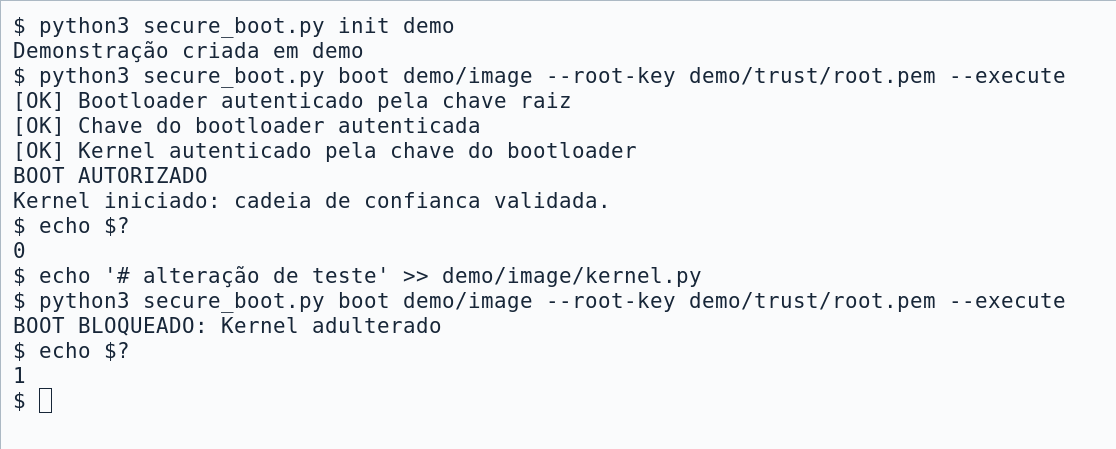
\includegraphics[width=\linewidth]{figuras/ensaio-simulador.png}
\end{figure}

Na primeira execução, o verificador autenticou o bootloader, a chave delegada e
o kernel. A mensagem emitida pelo próprio kernel e o código de saída 0
confirmaram a execução. Em seguida, acrescentamos a linha
\texttt{\# alteração de teste} ao arquivo \texttt{kernel.py}, em UTF-8 e com
uma quebra de linha ao final. O prefixo do SHA-256 passou de \texttt{d5886c53}
para \texttt{dd503567}. Na segunda execução, o verificador registrou
\texttt{Kernel adulterado} e devolveu o código 1.
A Figura~\ref{fig:simulador} mostra as duas chamadas com os mesmos argumentos.

Os 11 testes de \texttt{tests/test\_secure\_boot.py} passaram. A suíte exercitou,
entre outros casos, a troca da chave do bootloader, o uso de uma raiz incorreta,
assinaturas inválidas e arquivos ausentes. Um teste confirmou que o verificador
não iniciava o processo do kernel após uma falha. Outro comparou os bytes
enviados ao processo com os bytes verificados.

\clearpage
\section{Inicialização da máquina virtual}

A segunda parte do experimento usou QEMU 11.1.3, firmware OVMF e uma instalação
temporária do Linux From Scratch (LFS) 8.3~\cite{imagem-lfs}. O script
\texttt{vm/luks} provisionou uma máquina com duas CPUs virtuais, 2~GiB de RAM
e um disco raiz LUKS2. A imagem EFI assinada reunia o kernel Linux, o
\textit{initramfs} e os parâmetros de inicialização. O comando \texttt{sbverify}
confirmou sua assinatura com o certificado de teste. A inspeção do cabeçalho
com \texttt{cryptsetup luksDump} identificou AES-XTS e Argon2id.

Para testar a decisão do firmware, removemos a assinatura com \texttt{sbattach}
em uma cópia da imagem EFI. As variáveis de confiança do OVMF vieram da mesma
VM. O firmware tentou carregar o dispositivo, informou \texttt{Access Denied}
e esgotou as opções de inicialização (Figura~\ref{fig:firmware}). O fluxo
terminou antes do pedido de senha do disco.

\begin{figure}[H]
  \centering
  \caption{Recusa da imagem EFI sem assinatura pelo OVMF}
  \label{fig:firmware}
  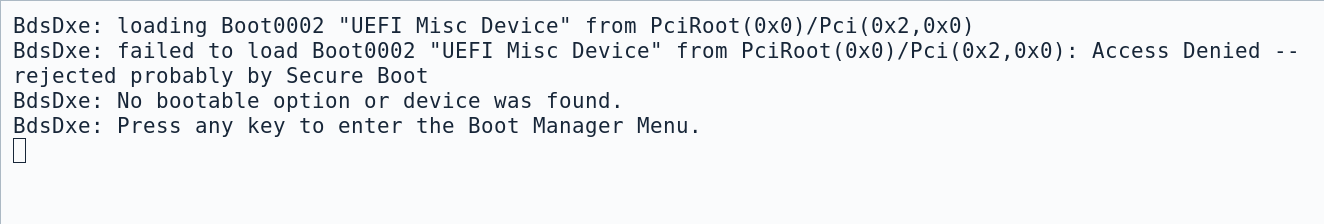
\includegraphics[width=\linewidth]{figuras/ensaio-firmware.png}
\end{figure}

Na segunda VM usamos o arquivo \texttt{lfs83.bz2} e o kernel
\texttt{7.3.5-arch1-1}. Assinamos a mesma imagem EFI com uma chave externa.
O \texttt{sbverify} retornou \texttt{Signature verification OK} ao
usar o respectivo certificado. Como a base \texttt{db} continuava com o
certificado original, o OVMF recusou a imagem antes do pedido de senha.

Com a imagem assinada pela chave autorizada, o firmware iniciou o kernel e o \textit{initramfs}
solicitou a senha do volume \texttt{t4root}. Ao receber uma senha incorreta, o
LUKS informou que nenhuma chave correspondia à senha e repetiu o pedido
(Figura~\ref{fig:luks}). Esta etapa já pertence ao Linux.

\begin{figure}[H]
  \centering
  \caption{Inicialização da imagem assinada e recusa da primeira senha pelo LUKS}
  \label{fig:luks}
  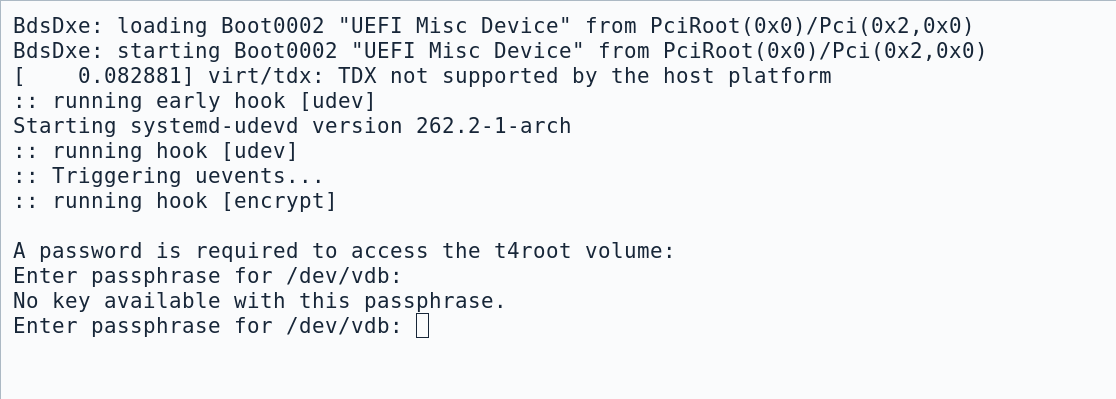
\includegraphics[width=\linewidth]{figuras/ensaio-luks.png}
\end{figure}

\clearpage
\section{Verificação no Linux inicializado}

Após o desbloqueio com a senha correta, entramos pelo console serial com a
conta \texttt{ensaio}. Em \texttt{/proc/mounts}, a entrada de \texttt{/}
mostrou que o dispositivo \texttt{/dev/mapper/t4root} fornecia a raiz ext4.
O arquivo de versão identificou o LFS 8.3
e \texttt{uname} retornou o kernel \texttt{7.3.5-arch1-1}. A leitura do
byte de dados da variável EFI \texttt{SecureBoot}, após os quatro bytes de
atributos, retornou 1 (Figura~\ref{fig:linux}).

\begin{figure}[H]
  \centering
  \caption{Versão do sistema, montagem da raiz e estado de Secure Boot no convidado}
  \label{fig:linux}
  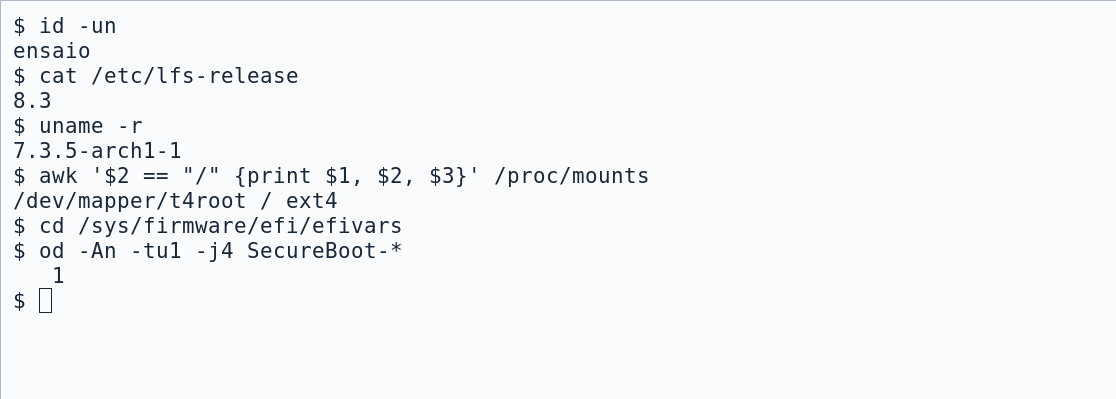
\includegraphics[width=0.88\linewidth,trim=0 45bp 0 0,clip]{figuras/ensaio-linux.png}
\end{figure}

Na VM reproduzida com \texttt{vm/luks prepare-lfs} e \texttt{vm/luks create},
entramos como \texttt{ensaio} e repetimos os comandos da Figura~\ref{fig:linux}.
A montagem da raiz e o estado do Secure Boot coincidiram com os do primeiro ensaio.
O teste \texttt{tests/luks\_vm.py} exercitou os quatro cenários com uma cópia
das variáveis originais do firmware a cada boot. A Figura~\ref{fig:testes}
reproduz as linhas de resultado emitidas pelo teste e pelo \texttt{sbverify}.

\begin{figure}[H]
  \centering
  \caption{Saída do teste de integração na VM com LFS 8.3}
  \label{fig:testes}
  \begin{minipage}{0.96\linewidth}
  \footnotesize
\begin{verbatim}
OK: o firmware recusou a imagem sem assinatura.
Signature verification OK
OK: o firmware recusou a imagem assinada por certificado externo.
OK: o LUKS recusou a senha incorreta.
OK: a imagem assinada chegou ao login com a senha correta.
\end{verbatim}
  \end{minipage}
\end{figure}

\section{Conclusão}

O comentário acrescentado ao kernel bastou para interromper a cadeia simulada.
Na VM, o OVMF recusou tanto a imagem sem assinatura quanto a assinada por uma
chave externa à base de confiança. A senha incorreta manteve o volume LUKS
fechado depois que o \textit{initramfs} já estava em execução. Com a imagem
assinada e a senha correta, o Linux montou a raiz cifrada e abriu uma sessão de
usuário. A assinatura verificada abrange a imagem EFI. A integridade individual
dos arquivos do ext4 e a revogação de chaves ficam fora destes ensaios.

\postextual
\nocite{assistente-ia}
\bibliography{referencias}

\section*{Declaração de uso de inteligência artificial}

\noindent\textbf{Simulador.} Utilizamos IA para implementar o simulador em Python
(\texttt{secure\_boot.py}). O programa gera os manifestos assinados com RSA-PSS
e verifica a cadeia de confiança da chave raiz até o kernel.

\smallskip
\noindent\textbf{Redação e documentação.} Em 23 de novembro de 2026, usamos um
assistente de programação da OpenAI para revisar o projeto à luz do enunciado.
A ferramenta revisou a introdução, calculou os hashes do kernel para o exemplo
que redigiu na seção~\ref{sec:exemplo-kernel} e escreveu o roteiro da VM no README.

\smallskip
\noindent\textbf{Código da VM.} O assistente implementou o comando
\texttt{vm/luks prepare-lfs}, que prepara a raiz ext4 e cria a conta de ensaio.
Acrescentou ao teste de integração o caso da imagem EFI assinada com uma chave
externa à base de confiança do firmware.

\smallskip
\noindent\textbf{Ensaios.} O assistente executou os 11 testes unitários existentes e
os quatro cenários de integração em uma VM criada a partir da imagem publicada
do LFS 8.3. A Figura~\ref{fig:testes} transcreve a saída dessa execução. Após
o login, a ferramenta também conferiu a montagem da raiz e leu o valor da
variável EFI \texttt{SecureBoot}.
\end{document}
